% mn2esample.tex
%
% v2.1 released 22nd May 2002 (G. Hutton)
%
% The mnsample.tex file has been amended to highlight
% the proper use of LaTeX2e code with the class file
% and using natbib cross-referencing. These changes
% do not reflect the original paper by A. V. Raveendran.
%
% Previous versions of this sample document were
% compatible with the LaTeX 2.09 style file mn.sty
% v1.2 released 5th September 1994 (M. Reed)
% v1.1 released 18th July 1994
% v1.0 released 28th January 1994

\documentclass[useAMS,usenatbib]{mn2e}
\usepackage{graphicx}
\usepackage{aas_macros}

% If your system does not have the AMS fonts version 2.0 installed, then
% remove the useAMS option.
%
% useAMS allows you to obtain upright Greek characters.
% e.g. \umu, \upi etc.  See the section on "Upright Greek characters" in
% this guide for further information.
%
% If you are using AMS 2.0 fonts, bold math letters/symbols are available
% at a larger range of sizes for NFSS release 1 and 2 (using \boldmath or
% preferably \bmath).
%
% The usenatbib command allows the use of Patrick Daly's natbib.sty for
% cross-referencing.
%
% If you wish to typeset the paper in Times font (if you do not have the
% PostScript Type 1 Computer Modern fonts you will need to do this to get
% smoother fonts in a PDF file) then uncomment the next line
% \usepackage{Times}

%%%%% AUTHORS - PLACE YOUR OWN MACROS HERE %%%%%


%%%%%%%%%%%%%%%%%%%%%%%%%%%%%%%%%%%%%%%%%%%%%%%%

\title[NEAT]{NEAT: Nebular Empirical Analysis Tool} %have to be the same?
\author[R. Wesson et al.]{R. Wesson$^{1,2}$, D.J. Stock$^{1,3}$ \& P. Scicluna$^{1,4}$\\
$^1$Department of Physics and Astronomy, University College London, Gower Street, London WC1E 6BT, UK\\
$^2$European Southern Observatory, Alonso de C ́rdova 3107, Casilla 19001, Santiago, Chile
$^3$Department of Physics and Astronomy, University of Western Ontario, London, Ontario, Canada, N6K 3K7\\
$^4$European Southern Observatory, Garching, Germany\\ %Peter, correct this
}


\begin{document}

\date{}

\pagerange{\pageref{firstpage}--\pageref{lastpage}} \pubyear{2002}

\maketitle

\label{firstpage}

\begin{abstract}
We present NEAT (Nebular Empirical Analysis Tool), a new code for calculating chemical abundances in photoionised nebulae.  The code carries out a standard analysis of lists of emission lines using long-established techniques to estimate the amount of interstellar extinction, calculate representative temperatures and densities, compute ionic abundances from both collisionally excited lines and recombination lines, and finally to estimate total elemental abundances using an ionisation correction scheme.

The code can be used to robustly calculate uncertainties on the derived abundances, via a Monte Carlo technique.  We show that for typical observational data, this approach is superior to analytic estimates of uncertainties, which inherently assume normally distributed uncertainties which are small relative to the quantity being measured.  These assumptions can break down severely for low signal-to-noise data.

We include in our analyses the effect of upward biasing on measurements of lines with low signal to noise, and we show that this effect (has whatever effect it has).

\end{abstract}

\begin{keywords}
Keywords
\end{keywords}

\section{Introduction}

Abundance determinations from photoionised nebulae play crucial roles in a variety of astrophysical contexts.  Galactic and extragalactic H~{\sc ii} regions provide vital constraints for galactic chemical evolution models; planetary nebulae provide constraints on theories of stellar nucleosynthesis and evolution; Wolf-Rayet ejecta nebulae reveal the effects of massive star recycling on the interstellar medium.

Such studies have a very long history (eg gratuitously ancient reference), but some major questions remain unanswered.  One long standing issue is the sometimes sizable discrepancy between abundances derived from collisionally excited lines (CELs) and those derived from recombination lines (RLs) - see for example recent papers by (a Liu, a Tsamis, a Wesson...).  One difficulty in understanding the significance of abundance data is that it is not trivial to realistically estimate the uncertainty on the derived quantities.  The final uncertainty will be due to both statistical uncertainty (ultimately deriving from the inherent uncertainty on the original line flux measurements) and systematic uncertainty (for example, the choice of reddening law or atomic data set).

In this paper we present a new code for calculating chemical abundances in photoionised nebulae, which can also robustly estimate statistical uncertainties using a Monte Carlo approach.  This method is inherently superior to analytic methods of uncertainty propagation.  We use our code to reanalyse several published line lists for which uncertainties are available, and we show that analytic methods can dramatically underestimate the true uncertainties on derived quantities.  For low signal to noise data, the true uncertainty distributions can be strongly non-Gaussian.

The words ``uncertainty" and ``error" are often used synonymously.  However, in this article we maintain the distinction in meaning between the terms: ``uncertainty" refers to the limiting accuracy of the knowledge of a quantity, while ``error" refers to an actual mistake.

\section{NEAT: Nebular empirical abundance tool}

\subsection{Input}

The new code, NEAT, largely builds upon previous codes, most importantly the {\sc equib} code (ref) for solving the equations of statistical equilibrium in multi-level atoms.  All the source code, documentation, atomic data and example line lists are freely available at \texttt{https://github.com/rwesson/NEAT}.


The code requires as input a plain text list of rest wavelengths, line fluxes, and uncertainties.  The user can then select the number of iterations of the code to run.  If the number of iterations is one, the code performs a standard empirical analysis on the line list, as described below, and does not calculate any uncertainties.  If the number of iterations is more than one, then the code first randomises the line list.  For each line, the code takes a random number from a Gaussian distribution with mean zero and standard deviation unity, multiplies this number by the line flux uncertainty, and adds it to the measured flux.  The standard analysis is then carried out on the randomised line list.

By carrying out this process many times, it is possible to build up an accurate picture of the true distribution of statistical uncertainties associated with the chemical abundances and empirical diagnostics resulting from the line flux uncertainties. The code collates all of the results from each iteration, and generates histograms showing visually the uncertainty distributions on the output parameters.

The code relies on the FORTRAN pseudo-random number generator, seeded using the system clock and the time of the code's exection.  The uniformly distributed numbers thus generated are then converted into a gaussian distribution.  We tested the performance of this approach by running the code 1\,000\,000 times, and plotting the distribution of fluxes obtained for an arbitrarily selected line.  We then fitted a gaussian function to this distribution.  We found that the recovered mean was within 0.008\% of the specified value, while the recovered standard deviation was within 0.13\% of the specified value.  Figure~\ref{gaussiantest} shows the histogram of generated values with the required gaussian distribution overplotted.  We thus consider that the random number generator in the code provides a reliably random Gaussian distribution.

\begin{figure}
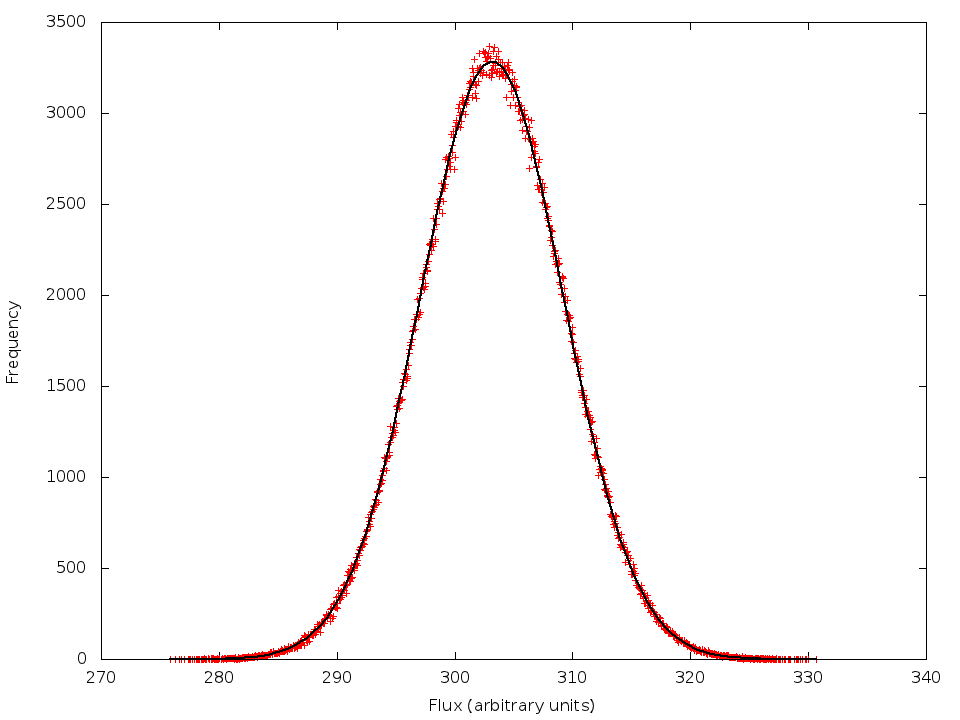
\includegraphics[width=0.47\textwidth]{figures/gaussian_test.png}
\caption{A distribution of values produced by 1\,000\,000 runs of the random number generator, with the target gaussian distribution overplotted.}
\label{gaussiantest}
\end{figure}

% eventually, do this:
\citet{1994A&A...287..676R} observed that measurements of weak lines (SNR$<$3) are strongly biased upwards.  For lines with F/$\sigma > $3, we account for this effect by taking the random number from a log-normal distribution with parameters determined... skewedness, mode...
%end

\subsection{Interstellar extinction}

The first step of any abundance analysis is a correction for interstellar extinction.  The amount of extinction is determined by NEAT from the ratios of hydrogen Balmer lines, and the user can select the particular extinction law to be used.  Five extinction laws are currently available: the Galactic extinction curves of \citet{1983MNRAS.203..301H}, \citet{1990ApJS...72..163F} and \citet{1989ApJ...345..245C}, the Large Magellanic Cloud law of \citet{1983MNRAS.203..301H}, and the Small Magellanic Cloud law of \citet{1984A&A...132..389P}.  In section~\ref{extinction} we investigate the effect on derived quantities of the likely uncertainty in $R$, the ratio of selective to total extinction.

\subsection{Temperatures and densities}

Temperatures and densities are calculated using traditional collisionally excited line diagnostics.  For the purposes of subsequent abundance calculations, the nebula is divided into three ``zones", of low, medium and high excitation.  In each zone, temperatures and densities are calculated iteratively and weighted according to the reliability of each diagnostic.  Table~\ref{zonestable} shows the diagnostics used and the weighting given in each zone.

\begin{table}
\begin{tabular}{ccc}
\hline
\multicolumn{3}{c}{Low ionisation zone}\\
\hline
Diagnostic & Lines & Weight \\
\hline
\multicolumn{3}{c}{Medium ionisation zone}\\
\hline
Diagnostic & Lines & Weight \\
\hline
\multicolumn{3}{c}{High ionisation zone}\\
\hline
Diagnostic & Lines & Weight \\
\end{tabular}
\label{zonestable}
\caption{Diagnostics used in the calculation of physical conditions.}
\end{table}

\subsection{Ionic abundances}

Ionic abundances are calculated from collisionally excited lines using the temperature and density appropriate to their ionisation potential.  Where several lines from a given ion are present, the ionic abundance adopted is found by averaging the abundances from each ion, weighting according to the observed intensity of the line.

Recombination lines are also used to derive ionic abundances.  In deep spectra, many more recombination lines may be available than collisionally excited lines.  The code first assigns IDs to each line based on their rest wavelengths, and then calculates the ionic abundance from the line intensity using the atomic data listed in Table~\ref{AD_reftable}.  Then, to determine the ionic abundance to adopt, it first derives an ionic abundance for each individual multiplet from the multiplet's co-added intensity, and then averages the abundances derived for each multiplet to obtain the ionic abundance used in subsequent calculations.

\subsection{Total elemental abundances}

Total elemental abundances are estimated using Ionisation Correction Factors.  The code includes the ICF scheme of \citet{1994MNRAS.271..257K}.

\section{Statistical uncertainties}

Uncertainties in observed quantities can be propagated into the uncertainty on derived parameters in a number of different ways, the two most common of which are the traditional analytical technique based on systems of partial derivatives and simplifying assumptions that allow one to apply Taylor expansions, and the `Monte Carlo' method which is a brute-force iterative method that exploits the wealth of computational power now readily available by building on knowledge of the uncertainty in the original observations.

The analytical approach is as follows: if one has measured a quantity $x$ with some uncertainty $\sigma x$, and wishes to calculate the uncertainty in a quantity $F$ given that $F = f(x)$, then the uncertainty on $F$ can be computed via the relation 

\begin{equation}
  \frac{\sigma F}{\sigma x} \simeq \frac{\partial f}{\partial x}
\end{equation}

However, in general one may not be able to compute this partial differential exactly, and in these cases, provided that

\begin{equation}
  \frac{\partial f}{\partial x}|_{x=x_1} \ll f(x_1)
\end{equation}

it is possible to use a first order Taylor expansion to approximate this derivative.  If one had a third value, $H = h(f, g)$ where $f$ and $g$ are both functions of other variables and are statistically independent of one another, it would be necessary to find the total derivative $dH$ such that

\begin{equation}
dh^2 = \left(\frac{\partial h}{\partial f}\right)^2df^2 + \left(\frac{\partial h}{\partial g}\right)^2dg^2
\end{equation}

and it thus follows that

\begin{equation}
\sigma^2_H = \left(\frac{\partial h}{\partial f}\sigma f\right)^2 + \left(\frac{\partial h}{\partial g}\sigma g\right)^2
\end{equation}

This expression can be generalised to any number of variables, and gives rise to the usual quadrature formulae for many simple functions of $x$.  We highlight three key aspects of this approach:

\begin{itemize}
  \item Given the number of formulae through which the original line flux data must be put before an abundance can be determined, and the wide variety of functions applied, the equations necessary to propagate uncertainties in this way can become extremely complex;
  \item the approach implicitly assumes that all the input and output uncertainties at each step are normally distributed;
  \item the Taylor expansion requires that the uncertainties be small relative to the quantities.
\end{itemize}

The first point is a matter of convenience but none the less one which discourages many authors from even attempting to propagate uncertainties all the way into the final quantities.  The second and third points are clearly violated in many or most real astrophysical observations, by virtue of which the uncertainties estimated using analytical techniques will be unreliable.


The Monte Carlo method, on the other hand, exploits the fact that an observation of a quantity $x$ is drawn from a distribution $X$, with mean $x$ and variance $\sigma_x$ . If one knows (or can make sensible assumptions about) the shape of this distribution, a random-number generator can be used to repeatedly draw values from X, creating a random sample from it. Using the above example of $F = f (x)$, if one wanted to examine the uncertainty in F , the operation f(x) could be performed upon every value in the aforementioned sample to produce a sample of the distribution from which F is drawn, which can then be parameterised to estimate the type, mean and standard deviation of this distribution. This process can be repeated ad infinitum for any number or combination of functions of F , x, or any other variable derived in the same way to propagate the uncertainties on the quantities, irrespective of the size of the uncertainties and any statistical interdependence of the variables.  This approach thus has the following advantages over the analytical approach:

\begin{itemize}
  \item It is inherently very simple;
  \item it requires no assumption about the particular distribution of uncertainties at any stage;
  \item it does not require relative uncertainties to be small
\end{itemize}

The Monte Carlo approach is thus inherently robust when applied to real astrophysical data, in a way that the analytical approach is not.  The only limitation is then the time taken to run the calculation enough times to sample well the statistics of the output distributions.

To demonstrate how traditional methods of uncertainty propagation do not properly reflect the true uncertainties on the derived chemical abundances, we briefly present here a reanalysis using NEAT of (an object with analytically calculated uncertainties).

%wo objects, along with the results from a third object which was originally analysed with NEAT (WR 18).  We chose objects having very deep, moderately deep and shallow spectra.  \citet{2011MNRAS.415..181F} presented a spectrum of NGC 7009 containing approximately 1300 identified emission lines.  NGC\,6543 \citep{2004MNRAS.351.1026W} has a spectrum with about 200 emission lines measured, and WR18 \citep{2011arXiv1108.3800S} has 36 lines detected.

%Discussions of Gaussian v. non-Gaussian distributions.  Bi-modal.  ICF complications.

\subsection{Non-Gaussian line flux uncertainties}

Rola and Pelat bit, how we incorporate it into NEAT, how it affects the uncertainties.

\subsection{Interstellar extinction}

We investigate the effect of the uncertainty in R, the ratio of total to selective extinction given by

\begin{equation}
R = \frac{A(V)}{E(B-V)}
\end{equation}

R is known to vary substantially along different sightlines (eg ref1, ref2), but estimating it for particular objects is generally impractical and instead, it is commonly assumed to equal 3.1.  We investigate the effect of an uncertainty in this value by comparing analyses in which R is fixed to be 3.1, and in which R is drawn from a Gaussian distribution with $\mu$=3.1 and $\sigma$=0.1.

\section{Discussion}

We have presented a new code for calculating chemical abundances in photoionised nebulae, which also robustly calculates the statistical uncertainties on the abundances determined.  We have used the code to show that analytic uncertainty propagation can dramatically underestimate the true uncertainties on abundances.

\section*{Acknowledgments}

We thank Professor Ian Howarth for useful discussions, Mahesh Mohan for testing an early version of the code, Bruce Duncan for helping us optimise the code, and the organisers of the workshop ``Uncertainties in atomic data and how they propagage in chemical abundances" for providing an extremely fruitful forum for interaction between atomic data providers and users.

\bibliographystyle{mn2e}
\bibliography{NEAT_paper}


\label{lastpage}

\end{document}
